\documentclass[math, info]{mpb-cours}

\title{Constructions à la Règle et au Compas}
\author{Matthieu Boyer}
\date{Cours TalENS 6 2025-2026}

\def\fC{\mathfrak{C}}
\def\fS{\mathfrak{S}}

\begin{document}
\bettertitle

Ce cours est basé sur \url{https://mathcircle.berkeley.edu/sites/default/files/handouts/2021/BMC_Adv_Constructions.pdf}

\section{Positionnement du Problème}

\begin{definition}
	Dans toute la suite, on désignera par \define{règle} un outil permettant de tracer et de prolonger des
	lignes droites infiniement parfaites passant par deux points, et par \define{compas} un outil
	permettant de tracer des cercles parfaits à partir de leur centre et d'un rayon.
\end{definition}

On s'intéresse au problème de construire des figures juste avec ces deux outils.
C'est la manière fondamentale qu'avait Euclide de faire des preuves: étant donné une série d'axiomes, de
constructions réalisables a priori, on sait définir la liste des constructions réalisables en général.

\begin{proposition}
	Sont constructibles:
	\begin{enumerate}
		\item La bissectrice d'un segment;
		\item La perpendiculaire à une droite passant par un point sur la droite;
		\item La perpendiculaire à une droite passant par un point hors de la droite;
		\item La bissectrice d'un angle;
		\item La parallèle à une droite passant par un point hors de la droite;
		\item Un triangle semblable à un autre triangle avec un côté prescrit;
		\item La subdivision d'un segment en $n$ parts égales pour $n \geq 1$.
	\end{enumerate}
\end{proposition}

Plus formellement, on va chercher à savoir quels nombres, quelles longueurs sont constructibles. Ici, on
identifiera le plan euclidien avec l'ensemble $\C$ des nombres complexes, mais ce n'est pas nécessaire pour
comprendre.

\begin{definition}
	Le \define{plan Euclidien} est l'espace vectoriel $\R^{2}$ muni de la base $(0, 1), (1, 0)$ et du produit
	scalaire la rendant orthonormale.
\end{definition}

En particulier, on notera

\begin{definition}[Axiomatique]
	On se suppose capable de faire les constructions suivantes:
	\begin{itemize}
		\item[R] Étant donnés deux points $z_{1}$, $z_{2}$ on peut tracer la droite passant par ces points.
		\item[C] Étant donné un point $z_{1}$ et deux points distincts $z_{2}, z_{3}$, on peut tracer le cercle
		      $\B(z_{1}, \abs{z_{2} - z_{3}})$ de centre $z_{1}$ et de rayon $\abs{z_{2} - z_{3}}$.
		\item[P\textsubscript{ll}] Étant données deux droites distinctes construites comme ci-dessus, on peut
		      construire leur point d'intersection.
		\item[P\textsubscript{lc}] Étant donnés une droite et un cercle construits comme ci-dessus, on peut
		      construire leurs points d'intersections.
		\item[P\textsubscript{cc}] Étant donnés deux cercles distincts construites comme ci-dessus, on peut
		      construire leurs points d'intersections.
	\end{itemize}
\end{definition}

\begin{definition}
	Le point $z \in \C$ est \define{constructible} s'il existe une suite finie d'opérations R, C,
	P\textsubscript{ll, lc, cc} qui commence avec les points $0, 1$ et qui termine en $z$.
	On note $\fC$ l'ensemble des nombres constructibles.
\end{definition}

\begin{exemple}
	Tout entier $m$ dans $\Z$ est constructible. Tout entier Gaussien $m + in \in \Z[i]$ est constructible.
	Les points $\frac{1}{2} \pm i \frac{\sqrt{3}}{2}$ sont constructibles.
\end{exemple}

\begin{proposition}
	$z$ est constructible si et seulement si son conjugué (symmétrique par rapport à la droite portant le
	segment $[0, 1]$) l'est.
\end{proposition}

\begin{thm}
	Le $n$-gone régulier est constructible si et seulement si le point $\xi_{n} = e^{2i\pi/n}$ l'est.
\end{thm}

La question qu'on se pose est donc la suivante: comment peut-on calculer $\fC$?

\section{Al-Jabr}
On va chercher une description algébrique de $\fC$, afin de savoir ce qui est constructible.

\subsection{Structures}

\begin{definition}
	Un \define{groupe} $(G, \cdot)$ est un ensemble $G$ muni d'une opération $\cdot$
	\begin{itemize}
		\item Associative: $(a\cdot b) \cdot c = a \cdot (b \cdot c)$ pour tous $a, b, c \in G$;
		\item Unifère: il existe un élément $e \in G$ tel que $e \cdot g = g \cdot e = g$ pour tout $g \in G$;
		\item Inversible: pour $g \in G$, il existe $g^{-1} \in G$ tel que $g \cdot g^{-1} = g^{-1}\cdot g = e$.
	\end{itemize}
	Un \define{morphisme} de groupes est une application préservant l'opération de groupe.
	On parle de \define{monomorphisme} si elle est injective, \define{epimorphisme} si elle est surjective, et
	d'\define{isomorphisme} si elle est bijective.
\end{definition}

\begin{exemple}
	$\Z, \Q, \R, \C$ sont des groupes pour l'addition. Ce ne sont pas des groupes pour la multiplication.

	On note $\fS_{A}$ le groupe des bijections $A \to A$ muni de la composition. Pour $A = \onen{n}$ on le
	note $\fS_{n}$.
\end{exemple}

\begin{thm}[Cayley]
	Tout groupe $G$ est isomorphe à un sous-groupe de $\fS_{G}$.
\end{thm}

\begin{definition}
	Un \define{anneau} est un groupe abélien pour l'addition de neutre $0$ muni d'une multiplication
	associative, commutative, unifère pour $1$ et distributive sur l'addition.
\end{definition}

\begin{exemple}
	$\Z, \Q, \R, \C$ sont des anneaux, $\znz{n}$ est un anneau pour l'addition et la multiplication modulo
	$n$.
\end{exemple}

\begin{definition}
	Si $R$ est un anneau, on note l'ensemble des polynômes à coefficients dans $R$ d'indéterminée $X$
	par
	\begin{equation*}
		R[X] = \left\{P = a_{0} + a_{1}X + a_{2}X^{2} + \cdots + a_{n}X^{n} \suchthat n \geq 0, a_{i} \in R \right\}
	\end{equation*}
	C'est aussi un anneau.
	Si $\alpha \in R$ et $P \in R[X] = \sum a_{i} X^{i}$, on note $P(\alpha) = \sum a_{i}\alpha^{i}$.
\end{definition}

\begin{definition}
	Un anneau est dit \define{intègre} s'il n'y a pas de diviseur de $0$, i.e. d'éléments non nuls dont
	le produit est nul.
\end{definition}

\begin{exemple}
	$\R$ est intègre, $\znz{5}$ est intègre, $\znz{6}$ ne l'est pas.
\end{exemple}

\begin{definition}
	Un \define{corps} est un anneau avec $1 \neq 0$ dont tous les éléments non nuls sont inversibles.
\end{definition}

\begin{exemple}
	$\Q, \R, \C$ sont des corps.
\end{exemple}

\begin{thm}
	$\znz{p}$ est un corps si et seulement si $p$ est premier.
\end{thm}

\begin{thm}
	L'ensemble $\fC$ est un corps. De plus:
	\begin{enumerate}
		\item $z = a +ib \in \fC$ si et seulement si $a \in \fC$ et $b \in \fC$ pour $a, b \in \R$;
		\item $z \in \fC \Rightarrow \sqrt{z} \in \fC$.
	\end{enumerate}
\end{thm}

\begin{remarque}
	Tout nombre complexe a deux racines carrées opposées, le deuxième point implique donc que les
	deux racines sont constructibles.
\end{remarque}

\begin{proof}
	Pour montrer que $\fC$ est un corps, nous devons montrer qu'il contient 0 et 1, qu'il est stable par
	addition et multiplication, qu'il contient l'opposé de chacun de ses éléments, et qu'il contient
	l'inverse multiplicatif de chacun de ses éléments non nuls.

	\begin{itemize}
		\item Par définition, $0 \in \fC$ et $1 \in \fC$.
		\item Soit $0 \neq z \in \fC$, $L(0, z)$ et $C(0, |z|)$ s'intersectent en $\pm z$. Donc $-z \in \fC$.
		\item Soient $z, w \in \fC$, alors la « règle du parallélogramme » nous indique comment construire
		      $z + w$ lorsque $0, z$ et $w$ ne sont pas colinéaires : $C(z, |w|)$ et $C(w, |z|)$ ont $z + w$
		      comme l'un de leurs points d'intersection. Lorsque $0, z$ et $w$ sont colinéaires,
		      il est encore plus facile de construire $z + w$. Ainsi $z + w \in \fC$.
	\end{itemize}

	Jusqu'ici, nous avons prouvé que $\fC$ est un groupe additif (et que $1 \in \fC$).

	Prouvons maintenant le premier point:
	Ensuite, si $z = a + ib \in \fC$, projetons orthogonalement $z$ sur les axes $x$ et $y$
	(ce qui est manifestement constructible).
	Nous obtenons $a \in \fC$ et $ib \in \fC$.
	Comme $C(0, |ib|)$ coupe l'axe des abscisses en $b$, on a $b \in \fC$.
	Réciproquement, si $a \in \fC$ et $b \in \fC$ (où $a, b \in \mathbb{R}$), alors $C(0, |b|)$ coupe l'axe
	des ordonnées en $ib$.
	Ainsi $ib \in \fC$ et par conséquent $z = a + ib \in \fC$ d'après ce que nous avons déjà démontré.

	\smallskip

	Pour prouver que $\fC$ est stable par multiplication et passage à l'inverse, nous allons d'abord prouver
	un résultat intermédiaire: $\fC \cap \{x \in \mathbb{R} \mid x > 0\}$ est stable par multiplication et
	passage à l'inverse.
	L'illustration suivante montre pourquoi cela est vrai.
	À partir de $a$ ou $b$, nous construisons $ia$ ou $ib$, puis nous traçons les droites parallèles
	appropriées, et nous raisonnons enfin avec des triangles semblables.

	% Section des graphiques TikZ
	\begin{center}
		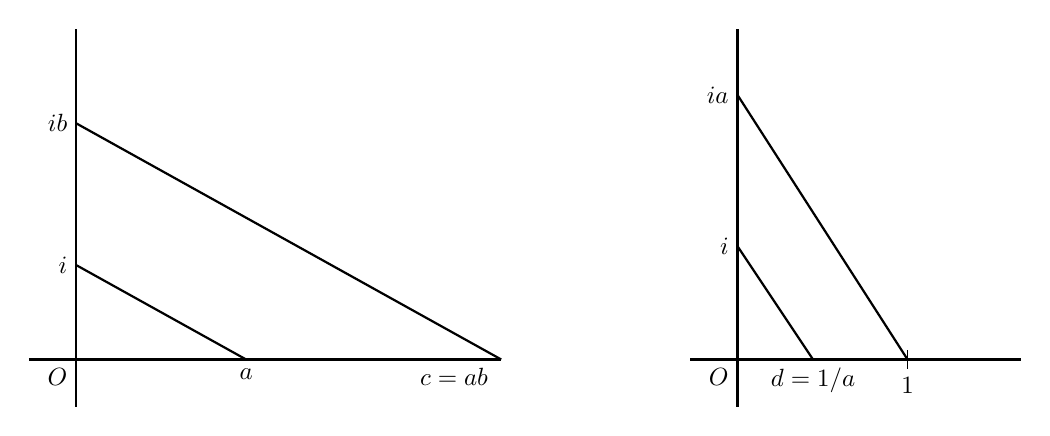
\begin{tikzpicture}[scale=1.2, >=stealth, every node/.style={scale=0.9}]

			% --- PREMIER GRAPHIQUE : MULTIPLICATION ---
			\begin{scope}[shift={(0,0)}]
				% Axes
				\draw[thick] (-0.5,0) -- (4.5,0); % Axe x
				\draw[thick] (0,-0.5) -- (0,3.5); % Axe y

				% Coordonnées
				\coordinate (O) at (0,0);
				\coordinate (I) at (0,1);
				\coordinate (IB) at (0,2.5);
				\coordinate (A) at (1.8,0);
				\coordinate (C) at (4.5,0); % Point c = ab calculé par Thalès

				% Droites (parallèles par construction)
				\draw[thick] (I) -- (A);
				\draw[thick] (IB) -- (4.5,0); % Ligne vers c = ab

				% Étiquettes
				\node[below left] at (O) {$O$};
				\node[left] at (I) {$i$};
				\node[left] at (IB) {$ib$};
				\node[below] at (A) {$a$};
				\node[below] at (4,0) {$c=ab$};
			\end{scope}

			% --- DEUXIÈME GRAPHIQUE : INVERSE ---
			\begin{scope}[shift={(7,0)}]
				% Axes
				\draw[thick] (-0.5,0) -- (3,0); % Axe x
				\draw[thick] (0,-0.5) -- (0,3.5); % Axe y

				% Coordonnées
				\coordinate (O) at (0,0);
				\coordinate (I) at (0,1.2);
				\coordinate (IA) at (0,2.8);
				\coordinate (D) at (0.8,0);
				\coordinate (ONE) at (1.8,0);

				% Droites (parallèles par construction)
				\draw[thick] (IA) -- (ONE);
				\draw[thick] (I) -- (D);

				% Étiquettes
				\node[below left] at (O) {$O$};
				\node[left] at (I) {$i$};
				\node[left] at (IA) {$ia$};
				\node[below] at (D) {$d=1/a$};
				\draw (1.8, -0.1) -- (1.8, 0.1); % Petit trait pour le 1
				\node[below] at (1.8, -0.1) {$1$};
			\end{scope}
		\end{tikzpicture}
	\end{center}
	Il en découle immédiatement que $\fC \cap \mathbb{R}$ est un corps.

	Nous pouvons maintenant montrer que $\fC$ est stable par multiplication et par l'inverse :
	Soient $z = a + ib \in \fC$ et $w = c + id \in \fC$. Alors $zw = (ac - bd) + i(ad + bc)$.
	En utilisant l'affirmation (a), puis le fait que $\fC \cap \mathbb{R}$ est un corps, et enfin
	de nouveau l'affirmation (a), il s'ensuit que $zw \in \fC$.
	De même, si $z \neq 0$, alors $\frac{1}{z} = \frac{a}{a^2+b^2} - i \frac{b}{a^2+b^2}$,
	et en utilisant le même raisonnement, nous voyons que $\frac{1}{z} \in \fC$.



	Il ne reste plus qu'à prouver l'affirmation (b) :
	Soit $0 \neq z \in \fC$.
	Écrivons $z = re^{i\theta}$ avec $0 < r = |z| \in \mathbb{R}$.
	Nous devons construire $w = \sqrt{r}e^{i\theta/2}$.
	Puisque $z \in \fC$, il est clair que nous pouvons construire un angle de mesure $\theta$.
	Comme nous pouvons diviser cet angle en deux (bissectrice), nous pouvons construire un angle
	de mesure $\theta/2$.
	Il est alors également clair que si nous pouvons construire $\sqrt{r}$, alors nous pouvons construire
	$w = \sqrt{z}$ et nous aurons terminé.
	Vous pouvez vérifier qu'il est possible de construire $\alpha$ comme dans la figure suivante et
	(en utilisant des triangles semblables) que le segment joignant $1$ à $\alpha$ a pour longueur $\sqrt{r}$.

	% Section du graphique TikZ : Racine carrée
	\begin{center}
		\begin{tikzpicture}[scale=1.5, >=stealth]
			% Axes
			\draw (-0.5,0) -- (3.5,0); % Axe horizontal
			\draw (0,-0.5) -- (0,2.5); % Axe vertical

			% Points clés
			\coordinate (O) at (0,0);
			\coordinate (ONE) at (1,0);
			\coordinate (R) at (2.5,0); % Point 1+r
			\coordinate (M) at (1.25,0); % Milieu du diamètre pour le cercle
			\coordinate (ALPHA) at (1,1.2247); % Point alpha sur le cercle (x=1, y=sqrt(r*1))

			% Le demi-cercle (diamètre 1+r = 2.5)
			\draw (2.5,0) arc (0:180:1.25);
			\draw (0,0) arc (180:345:1.25); % amorce du bas pour l'esthétique

			% Lignes de construction
			\draw (O) -- (ALPHA) -- (R);
			\draw (ONE) -- (ALPHA);

			% Symbole angle droit
			\draw (1,0.2) -- (1.2,0.2) -- (1.2,0);

			% Étiquettes et points
			\fill (O) circle (1.5pt) node[below left] {$O$};
			\fill (ONE) circle (1.5pt) node[below] {$1$};
			\fill (R) circle (1.5pt) node[below] {$1+r$};
			\fill (ALPHA) circle (1.5pt) node[above] {$\alpha$};

		\end{tikzpicture}
	\end{center}

	Par conséquent $\sqrt{z} \in \fC$ et la démonstration est terminée.
\end{proof}

\subsection{Polynômes}
Dans cette partie $R$ est un corps et on s'intéresse à des polynômes sur $R[X]$.
\begin{definition}
	Le \define{degré} d'un polynôme $P$ est la plus haute puissance de $X$ dans $P$. On le note $\deg P$.
\end{definition}

\begin{definition}
	La \define{division euclidienne} de $P'$ par $P$ est l'unique couple $(Q, R)$ tel que $P' = PQ + R$.
	On dit que $P$ \define{divise} $Q$ dans $R[X]$ quand $R = 0$.
	On note ceci $P \mid Q$.
	Un polynôme est \define{irréductible} s'il n'a pas de diviseur de degré $> 0$ autre que lui même.
\end{definition}

\begin{thm}
	Si $\deg P > 0$, alors $(t - \alpha) \mid P$ si et seulement si $P(\alpha) = 0$.
	On dit que $\alpha$ est une \define{racine} de $P$.
\end{thm}

\begin{thm}
	Dans $\C$, il n'y a pas de polynôme irréductible de degré $> 2$.
\end{thm}

\subsection{Extensions et Algébricité}
Dans la suite, $L$ et $K$ sont des corps.

\begin{definition}
	On dit que $L$ est une \define{extension du corps $K$} quand $K \subseteq L$, ce qu'on note $L:K$.
	On appelle le \define{degré} de l'extension $L:K$ ou \define{degré de $L$ sur $K$} la dimension de $L$
	comme $K$ espace vectoriel, on la note $[L:K]$.
\end{definition}

\begin{definition}
	Soit $K$ un corps et $X \subseteq K$. Le \define{sous-corps} de $K$ engendré par $X$ est le plus petit
	sous-corps de	$K$ contenant $X$. On le note $K(X)$.

	\smallskip

	Si $L:K$ est une extension de corps et $Y \subseteq L$, on note $K(Y)$ le sous-corps de $L$ engendré par
	$K \cup Y$.

	\smallskip

	L'extension $L:K$ est dite \define{simple} si $L = K(\alpha)$ pour un certain $\alpha \in L$.
\end{definition}

Par exemple, $\Q(\sqrt{2}) = \{p + q\sqrt{2} \mid p, q \in \Q\}$ et $\R(i) = \C$.
L'extension $\Q(i, \sqrt{5}):\Q$ est simple.


\begin{definition}
	Soit $L:K$ une extension de corps. $\alpha \in L$ est \define{algébrique} sur $K$ s'il existe un polynôme
	à coefficients dans $K$ non nul dont $\alpha$ est racine.
	Sinon, $\alpha$ est dit \define{transcendent}.

	\smallskip

	$L:K$ est une extension \define{algébrique} si tout élément de $L$ est algébrique sur $K$.
\end{definition}

\begin{definition}
	Soit $L:K$ une extension et $\alpha \in L$ algébrique sur $K$. Il existe un unique polynôme monique de
	plus petit degré dont $\alpha$ est racine.
	On l'appelle le \define{polynôme minimal} de $\alpha$ sur $K$ et on le note $m_{\alpha}$.
\end{definition}

\begin{thm}
	On a $[K(\alpha):K] = \infty$ si $\alpha$ est transcendent sinon $[K(\alpha):K] = \deg m_{\alpha}$.
\end{thm}

\begin{proposition}
	Si $K_{0} \subseteq K_{1} \subseteq \cdots \subseteq K_{n}$ sont des corps, alors
	\begin{equation*}
		[K_{n}:K_{0}] = \prod_{i = 0}^{n-1} [K_{i + 1}:K_{i}].
	\end{equation*}
\end{proposition}

\begin{proposition}
	Si $L:K$ est une extension de degré $2$, alors $L = K(\sqrt(\alpha))$ pour $\alpha \in K$.
\end{proposition}

\begin{definition}
	La clôture pythagoréenne $\Q^{py}$ de $\Q$ est le plus petit sous-corps de $\C$ stable par racine.
\end{definition}

\begin{thm}
	$\fC = \Q^{py}$
\end{thm}
\begin{proof}
	On vérifie simplement l'inclusion $\fC \subseteq \Q^{py}$.
	Tout $z \in \fC$ est obtenue par une suite finie de constructions à partir de $0$ et $1$.
	Chaque point construit peut se voir comme une solution d'un système d'équations qui s'expriment avec des
	opérations de corps et des racines carrées à partir des points précédents.
\end{proof}

\begin{thm}
	On a $z \in \fC$ si et seulement si il existe une suite d'extensions de $\Q$ par des sous-corps $K_{i}$
	de $\C$ tel que $z \in K_{n}$ et $[K_{i}:K_{i-1}] = 2$
\end{thm}

\begin{proof}
	Pour montrer que la condition est suffisante, on vérifie par récurrence que $K_{i} \subseteq \fC$.
	Puisque $K_{i} = K_{i - 1}(\sqrt{\alpha})$ pour un certain $\alpha \in K_{i - 1}$, $\alpha \in \fC$.
	De plus $\sqrt{\alpha} \in \fC$ et donc $K_{i} \subseteq \fC$.

	Réciproquement, puisque $\fC = \Q^{py}$, $z$ peut s'obtenir par une suite finie d'opérations de corps
	et de racines. Chaque étape dans cette suite peut se faire soit au sein d'un même corps soit par une
	extension de la forme $K_{i} = K_{i - 1}(\sqrt{\alpha})$ qui produit une extension de degré $2$.
\end{proof}

\begin{corollaire}
	Si $\alpha \in \fC$, alors $[\Q(\alpha):\Q] = \deg m_{\alpha} = 2^m$ pour $m\geq 0$.
\end{corollaire}

\subsection{Quelques résultats en conséquence}
\begin{proposition}
	Le cube ne peut pas être doublé à la règle et au compas.
\end{proposition}
\begin{proof}
	Doubler le cube équivaut à construire $\alpha = \sqrt[3]{2} \in \R$, donc le polynôme minimal est
	$X^{3} - 2$. En particulier, $[\Q(\alpha):\Q] = 3$ et donc $\alpha \notin\fC$.
\end{proof}

\begin{proposition}
	La quadrature du cercle est impossible à la règle et au compas.
\end{proposition}
\begin{proof}
	La quadrature du cercle équivaut à la construction de $\sqrt{\pi}$.
	Si $\sqrt{\pi} \in \fC$ alors $\pi \in \fC$ et donc $\pi$ est algébrique, ce qui n'est pas vrai.
\end{proof}

\begin{proposition}
	La trisection de l'angle n'est pas faisable à la règle et au compas.
\end{proposition}
\begin{proof}
	L'angle de mesure $2\pi/3$ n'est pas trisectable. Cela reviendrait à construire $\xi_{9} = e^{2i\pi/9}$.
	Si $\xi_{9} \in \fC$, alors $\alpha = \xi_{9} + \xi_{9}^{-1} \in \fC$.
	Or, $\alpha$ est une racine de $X^{3} -3X + 1 \in \Q[X]$, qui est irréductible sur $\Q$ et est donc son
	polynôme minimal, qui n'est pas de degré une puissance de $2$.
\end{proof}

\begin{proposition}
	Soit $n > 2$ un entier. Le $n$-gone régulier peut être construit à la règle et au compas si et seulement
	si $n = 2^{r}p_{1}\ldots p_{s}$ où $r \geq 0$, $s\geq 0$ et les $p_{i}$ sont des premiers de Fermat de la
	forme $p = 2^{2^{k}} + 1$.
\end{proposition}

\end{document}
